\documentclass[a4paper, 12pt]{article}

% Essential packages
\usepackage[T1, T2A]{fontenc}
\usepackage[utf8]{inputenc}
\usepackage[russian, english]{babel}
\usepackage{graphicx}
\usepackage{geometry}
\usepackage{amsmath}
\usepackage{amsfonts}
\usepackage{amssymb}
\usepackage{hyperref}
\usepackage{indentfirst}
\usepackage{authblk}
\usepackage{gensymb}
\usepackage{listings}
\usepackage{xcolor}
\usepackage{minted}
\usepackage{float}
\usepackage{caption}
\usepackage[russian]{babel}

\captionsetup[figure]{name=Рис., aboveskip=0.5pt, belowskip=0.5pt}


\captionsetup[table]{name=Табл., aboveskip=1pt, belowskip=0.5pt}

\setminted{
    breaklines=true,
    breakautoindent=true,
    breakindent=20pt,
    fontsize=\small,  % опционально: уменьшает шрифт
    frame=lines,      % опционально: рамка для наглядности
    framesep=2mm
}

% \lstset{
%     language=Matlab,
%     basicstyle=\ttfamily\small,
%     numbers=left,
%     numberstyle=\tiny,
%     stepnumber=1,
%     breaklines=true,
%     keywordstyle=\color{blue},
%     commentstyle=\color{green!50!black},
%     stringstyle=\color{red},
%     frame=single
% }

% Page margins setup
\geometry{left=2cm, right=2cm, bottom=2cm, top=2cm}

% Hyperlink setup
\hypersetup{
    colorlinks=true,
    linkcolor=blue,
    filecolor=magenta,
    urlcolor=cyan
}

\begin{document}
\begin{titlepage}

\begin{minipage}[c]{0.65\textwidth}
    {\vspace{0.5cm}\Large\textbf{УНИВЕРСИТЕТ ИТМО}}\\
    \small{Факультет Систем Управления и Робототехники}
\end{minipage}
\begin{minipage}[c]{0.35\textwidth}
    \begin{flushright}
        
\includegraphics[width=0.8\textwidth]{itmo.png}
    \end{flushright}
\end{minipage}

\vfill
\vfill

\begin{center}
\textbf{\Large Лабораторная работа №1 <<Ряды Фурье>>}\\[5pt]
{\large Частотные методы}


\vfill
\vfill

\begin{flushleft}
    Выполнили:\\
    \text{Бурдасова Виктория: 465306}\\
    \text{Жаворонков Пётр: 465877}\\
    \text{Беляев Александр: 465203}
\end{flushleft}

\vfill

Санкт-Петербург\\
2026

\end{center}
\end{titlepage}
\renewcommand*\contentsname{Содержание}
\tableofcontents

\newpage
\section{Вещественные функции}
Задание: Задаться числами $a,\ b,\ t_0,\ t_1,\ t_2$ такими, что $a,\ b > 0$ и $t_2 > t_1 > t_0 > 0$.
Рассмотреть следующие функции $f : \mathbb{R} \to \mathbb{R}$:

\begin{enumerate}
    \item \textbf{Квадратная волна} --- периодическая функция с периодом $T = t_2 - t_0$ такая, что
    \[
    f(t) =
    \begin{cases}
        a, & t \in [t_0, t_1), \\
        b, & t \in [t_1, t_2).
    \end{cases}
    \]
    
    \item \textbf{Чётная} периодическая функция, которая не может быть 
    представлена конечным числом членов ряда Фурье, на ваш выбор.

    \item \textbf{Нечётная} периодическая функция, которая не может быть 
    представлена конечным числом членов ряда Фурье, на ваш выбор.

    \item Периодическая функция, которая не может быть представлена 
    конечным числом членов ряда Фурье и которая не является 
    ни чётной, ни нечётной, на ваш выбор.
\end{enumerate}

Также для каждой из функций необходимо рассмотреть частичные суммы рядов Фурье $F_N$ и $G_N$ вида:
\[
F_N(t) = \frac{a_0}{2} + \sum_{n=1}^{N}
\left( a_n \cos(\omega_n t) + b_n \sin(\omega_n t) \right),
\] 

\[
G_N(t) = \sum_{n=-N}^{N} c_n e^{i \omega_n t},
\]

где $\omega_n = \dfrac{2\pi n}{T}$.\\

Для этого:

\begin{enumerate}
    \item Проанализировать рассматриваемые функции и определить,
    очевидны ли значения некоторых коэффициентов.

    \item Написать программу для вычисления коэффициентов рядов Фурье
    $(a_n, b_n)$ и $c_n$ для произвольного $N$.
    Привести в отчёте полученные коэффициенты при $N = 2$.
    Проверить, подтвердились ли догадки.

    \item Задаться пятью различными значениями $N$ и построить графики
    $F_N(t)$ и $G_N(t)$.
    Сравнить их друг с другом и с графиком исходной функции $f(t)$:
    для каждого значения $N$ на одном рисунке должен быть приведён
    набор графиков $F_N(t)$, $G_N(t)$ и $f(t)$ на одной координатной
    плоскости.

    \item Выбрать наибольшее из рассмотренных $N$ и проверить выполнение
    равенства Парсеваля для оригинала функции $f(t)$ и рассмотренных
    частичных сумм ряда $F_N(t)$ и $G_N(t)$.
    При проверке равенства приводить формулы, по которым осуществляется
    проверка. Объяснить разницу между величинами.
\end{enumerate}



В данной работе рассмотрены разложения следующих порядков: $N = {2,\ 3,\ 10,\ 20,\ 50}$.

Ввиду того, что применение равенства Парсеваля корректно только в случае рядов Фурье (бесконечных сумм), в данной лабораторной работе вводится понятие \textbf{примерного равенства Парсеваля} для частичных сумм:
\[
\frac{1}{T}\int_{t_0}^{t_0+T} f^2(t)\,dt \approx \sum_{n=-N}^{N} |c_n|^2,
\]
В примерном равенстве Парсеваля объектом исследования является абсолютная ошибка $\Delta$ этого примерного равенства: чем она меньше, тем лучше частичная сумма аппроксимирует данную функцию.

\subsection{Квадратная волна}
Выберем коэффициенты. Пусть a = 12; b = 6; $t_0$ = 1; $t_1$ = 2; $t_2$ = 3;\\

\[
    f(t) =
    \begin{cases}
        12, & t \in [1, 2), \\
        6, & t \in [2, 3).
    \end{cases}
\]\\

Её период равен $T = t_2 - t_0 = 3 - 1 = 2$, а график выглядит так:
\begin{figure}[H] 
    
\includegraphics[width=1\textwidth]{images/graphs/figure_1.pdf}
    \caption{График квадратной волны, отражающий 3 периода}
\end{figure}

Теперь рассмотрим частичные суммы этой функции вида:

\[
F_N(t) = \frac{a_0}{2} + \sum_{n=1}^{N}
\left( a_n \cos(\omega_n t) + b_n \sin(\omega_n t) \right),
\]

\[
G_N(t) = \sum_{n=-N}^{N} c_n e^{i \omega_n t},
\]

где $\omega_n = \dfrac{2\pi n}{T}$.\\

Коэффициенты $a_n$, $b_n$ и $c_n$ вычисляются по формулам:

\[
a_n = \frac{1}{\pi}\int_{-\pi}^{\pi}f(t)\cos(nt)dt
\]
\[
b_n = \frac{1}{\pi}\int_{-\pi}^{\pi}f(t)\sin(nt)dt
\]
\[
c_n = \frac{1}{2\pi}\int_{-\pi}^{\pi}f(t)(\cos(nt)-i\sin(nt))dt=
\frac{1}{2\pi}\int_{-\pi}^{\pi}f(t)e^{-int}dt
\]

С помощью программы найдём коэффициенты $a_n$, $b_n$ и $c_n$ при N = 2:\\
$a_0=18.00$\\
$a_1=-0.00; b_1=-3.82$\\
$a_2=0.00; b_2=-0.00$\\
$c_-2=0.00-0.00j$\\
$c_-1=-0.00-1.91j$\\
$c_0=9.00$\\
$c_1=-0.00+1.91j$\\
$c_2=0.00+0.00j$\\

Зададимся следующими значениями $N = {2,\ 3,\ 10,\ 20,\ 50}$.

Теперь рассмотрим графики $F_N(t)$ и $G_N(t)$ для каждого $N$:

\begin{figure}[H] 
    
\includegraphics[width=1\textwidth]{images/graphs/figure_2.pdf}
    \caption{Графики $F_N(t)$ и $G_N(t)$ при N=2}
\end{figure}

\begin{figure}[H] 
    
\includegraphics[width=1\textwidth]{images/graphs/figure_3.pdf}
    \caption{Графики $F_N(t)$ и $G_N(t)$ при N=3}
\end{figure}

\begin{figure}[H] 
    
\includegraphics[width=1\textwidth]{images/graphs/figure_4.pdf}
    \caption{Графики $F_N(t)$ и $G_N(t)$ при N=10}
\end{figure}

\begin{figure}[H] 
    
\includegraphics[width=1\textwidth]{images/graphs/figure_5.pdf}
    \caption{Графики $F_N(t)$ и $G_N(t)$ при N=20}
\end{figure}

\begin{figure}[H] 
    
\includegraphics[width=1\textwidth]{images/graphs/figure_6.pdf}
    \caption{Графики $F_N(t)$ и $G_N(t)$ при N=50}
\end{figure}



\textbf{Проверка примерного равенства Парсеваля}

Для данной функции $f(t)$ с периодом $T = 2$ примерное равенство Парсеваля имеет вид:
\[
\frac{1}{2}\int_{1}^{3} f^2(t)dt \approx \sum_{n=-N}^{N} |c_n|^2
\]
Проверим оценку для максимального рассмотренного $N = 50$:

\begin{table}[H]
\centering
\begin{tabular}{|l|c|}
\hline
\textbf{Величина} & \textbf{Значение} \\
\hline
Левая часть $\displaystyle\frac{1}{2}\int_{1}^{3} f^2(t)dt$ & 90.000000 \\
Правая часть $\displaystyle\sum_{n=-50}^{50} |c_n|^2$ & 89.927058 \\
Абсолютная ошибка $\Delta$ & $7.294 \times 10^{-2}$ \\
\hline
\end{tabular}
\caption{Проверка примерного равенства Парсеваля при $N = 50$ для квадратной волны}
\end{table}

\textbf{Анализ:} Для данной функции абсолютная ошибка на 2 порядка меньше, чем значения левой и правой частей равенств.

\subsection{Чётная периодическая функция.}
Зададим следующую чётную периодическую функцию:\\

\[
    f(t) =
    \begin{cases}
        4\cdot t + 12, & t \in [-3, -2), \\
        -2\cdot t, & t \in [-2, -1),\\
        2, & t \in [-1, 1),\\
        2\cdot t, & t \in [1, 2),\\
        -4\cdot t + 12, & t \in [2, 3),
    \end{cases}
\]\\

Её период равен $T = t_2 - t_0 = 3 - (-3) = 6$, а график выглядит так:
\begin{figure}[H] 
\centering
\begin{tabular}{ll}

\includegraphics[scale=0.6]{images/graphs/figure_8.pdf}
\end{tabular}
\caption{График чётной периодической функции, отражающий 3 периода}
\end{figure}

Теперь рассмотрим частичные суммы этой функции. Очевидно, что коэффициент $b_n = 0$, потому что рассматриваемая функция $f(t)$ чётная, а функция синуса --- нечётная. 

Смотрим на результаты выполнения программы для этой функции при $N = 2$:\\
$a_0=4.67$\\
$a_1=0.00; b_1=0.00$\\
$a_2=-0.91; b_2=0.00$\\
$c_{-2}=-0.46-0.00j$\\
$c_{-1}=0.00+0.00j$\\
$c_0=2.33$\\
$c_1=0.00-0.00j$\\
$c_2=-0.46+0.00j$\\

Догадки по поводу коэффициента $b_n$ подтвердились: он действительно равен 0.

Теперь рассмотрим графики $F_N(t)$ и $G_N(t)$ для каждого $N$:

\begin{figure}[H] 
\centering
\begin{tabular}{ll}

\includegraphics[scale=0.6]{images/graphs/figure_9.pdf}
\end{tabular}
\caption{График частичных сумм при N = 2}
\end{figure}

\begin{figure}[H] 
\centering
\begin{tabular}{ll}

\includegraphics[scale=0.6]{images/graphs/figure_10.pdf}
\end{tabular}
\caption{График частичных сумм при N = 3}
\end{figure}

\begin{figure}[H] 
\centering
\begin{tabular}{ll}

\includegraphics[scale=0.6]{images/graphs/figure_11.pdf}
\end{tabular}
\caption{График частичных сумм при N = 10}
\end{figure}

\begin{figure}[H] 
\centering
\begin{tabular}{ll}

\includegraphics[scale=0.6]{images/graphs/figure_12.pdf}
\end{tabular}
\caption{График частичных сумм при N = 20}
\end{figure}

\begin{figure}[H] 
\centering
\begin{tabular}{ll}

\includegraphics[scale=0.6]{images/graphs/figure_13.pdf}
\end{tabular}
\caption{График частичных сумм при N = 50}
\end{figure}

\textbf{Проверка примерного равенства Парсеваля}

Для данной функции $f(t)$ с периодом $T = 6$ примерное равенство Парсеваля имеет вид:
\[
\frac{1}{6}\int_{-3}^{3} f^2(t)dt \approx \sum_{n=-N}^{N} |c_n|^2
\]
Проверим оценку для максимального рассмотренного $N = 50$:

\begin{table}[H]
\centering
\begin{tabular}{|l|c|}
\hline
\textbf{Величина} & \textbf{Значение} \\
\hline
Левая часть $\displaystyle\frac{1}{6}\int_{-3}^{3} f^2(t)dt$ & 6.222222 \\
Правая часть $\displaystyle\sum_{n=-50}^{50} |c_n|^2$ & 6.222203 \\
Абсолютная ошибка $\Delta$ & $1.885 \times 10^{-5}$ \\
\hline
\end{tabular}
\caption{Проверка примерного равенства Парсеваля при $N = 50$ для чётной периодической функции}
\end{table}

\textbf{Анализ:} Для данной функции значение ошибки на 5 порядков меньше значений левой и правой частей.

\newpage\subsection{Нечётная периодическая функция (Пилообразная волна)}
В общем виде пилообразная волная задаётся следующим выражением:
$$f(t) = \frac{2A}{T}\cdot t,\;\;\;t\in[-\frac{T}{2};\frac{T}{2}]$$

Коэффициент А отвечает за амплитуду, T --- период. Выберем параметры: $A = 7$, $T = 2\pi\approx 6.28$. Тогда:
$$f(t) = \frac{14t}{2\pi} = \frac{7t}{\pi}$$

График этой функции на отрезке [-T; 2T] можно увидеть на рисунке~\ref{fig:pic11}.


\begin{figure}[H]
    \centering
    
\includegraphics[width=1\linewidth]{images/graphs/figure_15.pdf}
    \caption{График пилообразной волны, отражающий 3 периода}
    \label{fig:pic11}
\end{figure}

Так как функция подбиралась как нечётная, в разложении Фурье будет отсутствовать косинус-составляющая, следовательно все коэффициенты $a_i\equiv0,\;\;i=1...N$. Если рассмотреть график функции только на одном периоде, можно заметить, что он симметричен относительно точки пересечения с осью ординат, то есть среднее значение сигнала будет лежать на этой оси, следовательно $a_0=0$.

Вывод программы для этой функции при $N=2$:
\begin{minted}{text}
[CFC] For real Fourier:
[CFC] a_0=-0.00
[CFC] a_1=2.8271597168564594e-16; b_1=4.456338406573071
[CFC] a_2=-4.598774148841224e-16; b_2=-2.228169203286535
[CFC] For complex Fourier:
[CFC] c_-2=(-2.299387074420612e-16-1.1140846016432675j)
[CFC] c_-1=(1.4135798584282297e-16+2.2281692032865354j)
[CFC] c_0=-2.8271597168564594e-16
[CFC] c_1=(1.4135798584282297e-16-2.2281692032865354j)
[CFC] c_2=(-2.299387074420612e-16+1.1140846016432675j)
\end{minted}

Видим, что значение коэффициентов $a_n$ на 16 порядков меньше, чем значения $b_n$, то есть влияние косинусоид настолько мало, что его можно считать нулевым. 

Для всех выбранных N получились следующие графики:
\begin{figure}[H] 
    
\includegraphics[width=1\textwidth]{images/graphs/figure_16.pdf}
    \caption{Графики $F_N(t)$ и $G_N(t)$ при N=2}
\end{figure}

\begin{figure}[H] 
    
\includegraphics[width=1\textwidth]{images/graphs/figure_17.pdf}
    \caption{Графики $F_N(t)$ и $G_N(t)$ при N=3}
\end{figure}

\begin{figure}[H] 
    
\includegraphics[width=1\textwidth]{images/graphs/figure_18.pdf}
    \caption{Графики $F_N(t)$ и $G_N(t)$ при N=10}
\end{figure}

\begin{figure}[H] 
    
\includegraphics[width=1\textwidth]{images/graphs/figure_19.pdf}
    \caption{Графики $F_N(t)$ и $G_N(t)$ при N=20}
\end{figure}

\begin{figure}[H] 
    
\includegraphics[width=1\textwidth]{images/graphs/figure_20.pdf}
    \caption{Графики $F_N(t)$ и $G_N(t)$ при N=50}
\end{figure}

\textbf{Проверка примерного равенства Парсеваля}

Для данной функции $f(t) = \frac{7t}{\pi}$ с периодом $T = 4\pi$ примерное равенство Парсеваля имеет вид:
\[
\frac{1}{2\pi}\int_{-\pi}^{\pi} \left(\frac{7t}{\pi}\right)^2dt \approx \sum_{n=-N}^{N} |c_n|^2
\]
Проверим оценку для максимального рассмотренного $N = 50$:

\begin{table}[H]
\centering
\begin{tabular}{|l|c|}
\hline
\textbf{Величина} & \textbf{Значение} \\
\hline
Левая часть $\displaystyle\frac{1}{2\pi}\int_{-\pi}^{\pi} \left(\frac{7t}{\pi}\right)^2dt$ & 16.333333 \\
Правая часть $\displaystyle\sum_{n=-50}^{50} |c_n|^2$ & 16.136716 \\
Абсолютная ошибка $\Delta$ & $1.966 \times 10^{-1}$ \\
\hline
\end{tabular}
\caption{Проверка примерного равенства Парсеваля при $N = 50$ для пилообразной волны}
\end{table}

\textbf{Анализ:} Для данной функции ошибка имеет порядок на 1 меньше, чем порядок значений левой и правой частей.

\subsection{Периодическая функция (ни чётная, ни нечётная)}
Рассмотрим периодическую функцию вида:
$$f(t) = (1-\pi)^2 \sin(t) + t, \quad t \in [0, T)$$

где период $T = 4\pi \approx 12.57$.

3 периода данной функции выглядят следующим образом:

\begin{figure}[H]
    \centering
    
\includegraphics[width=1\linewidth]{images/graphs/figure_22.pdf}
    % \caption{График функции, отражающий 3 периода}
    \label{fig:placeholder}
\end{figure}

Так как функция не является ни чётной, ни нечётной, так как помимо синуса содержит полиномиальную часть, в разложении Фурье будут присутствовать как косинусоидальные, так и синусоидальные компоненты, однако синус присутствует в выражении явно, а косинус --- нет, поэтому вероятно коэффициент при косинусе будет сильно меньше, чем при синусе. При этом функция полностью находится в положительной по вертикальной оси части плоскости, значит $\displaystyle 0\le \frac{a_0}{2}\le sup(f)$.

Вывод программы для этой функции при $N=2$:

\begin{minted}{text}
[CFC] For real Fourier:
[CFC] a_0=12.57
[CFC] a_1=9.979426752319347e-17; b_1=-4.000000000000001
[CFC] a_2=-1.6606481500369727e-15; b_2=2.5864190939097713
[CFC] For complex Fourier:
[CFC] c_-2=(-8.303240750184864e-16+1.2932095469548857j)
[CFC] c_-1=(4.9897133761596735e-17-2.0000000000000004j)
[CFC] c_0=6.283185307179585
[CFC] c_1=(4.9897133761596735e-17+2.0000000000000004j)
[CFC] c_2=(-8.303240750184864e-16-1.2932095469548857j)
\end{minted}

Для данной функции значения $a_n$ на 17 и 15 порядков соответственно меньше значений $b_n$. В целом расчёты подтверждают анализ, однако ожидалось, что разность порядков будет по крайней мере меньше, чем в прошлом примере, где вклад косинусоиды приравнивается к нулю.

Для всех выбранных N получились следующие графики:
\begin{figure}[H] 
    
\includegraphics[width=1\textwidth]{images/graphs/figure_23.pdf}
    \caption{Графики $F_N(t)$ и $G_N(t)$ при N=2}
\end{figure}

\begin{figure}[H] 
    
\includegraphics[width=1\textwidth]{images/graphs/figure_24.pdf}
    \caption{Графики $F_N(t)$ и $G_N(t)$ при N=3}
\end{figure}

\begin{figure}[H] 
    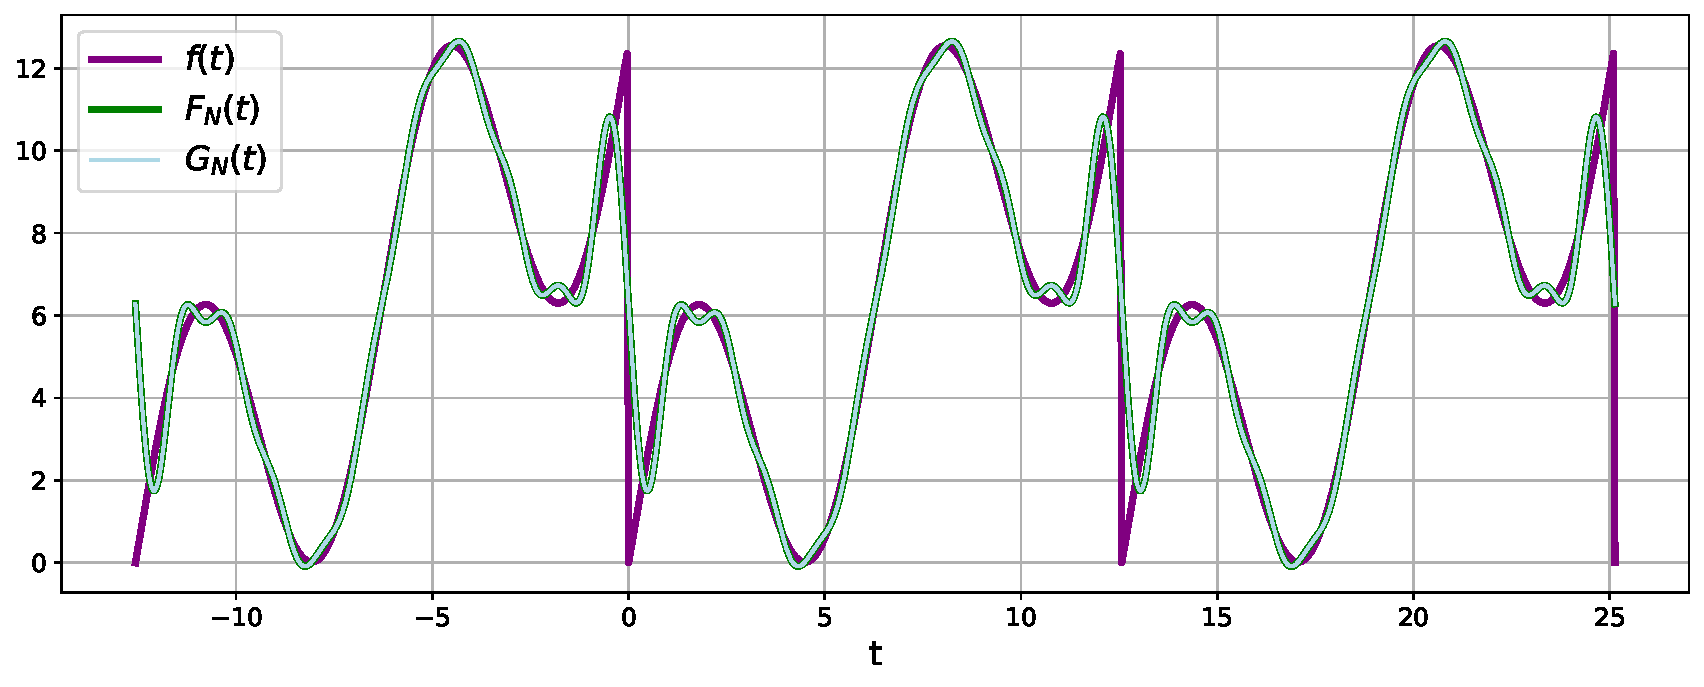
\includegraphics[width=1\textwidth]{images/graphs/figure_25.pdf}
    \caption{Графики $F_N(t)$ и $G_N(t)$ при N=10}
\end{figure}

\begin{figure}[H] 
    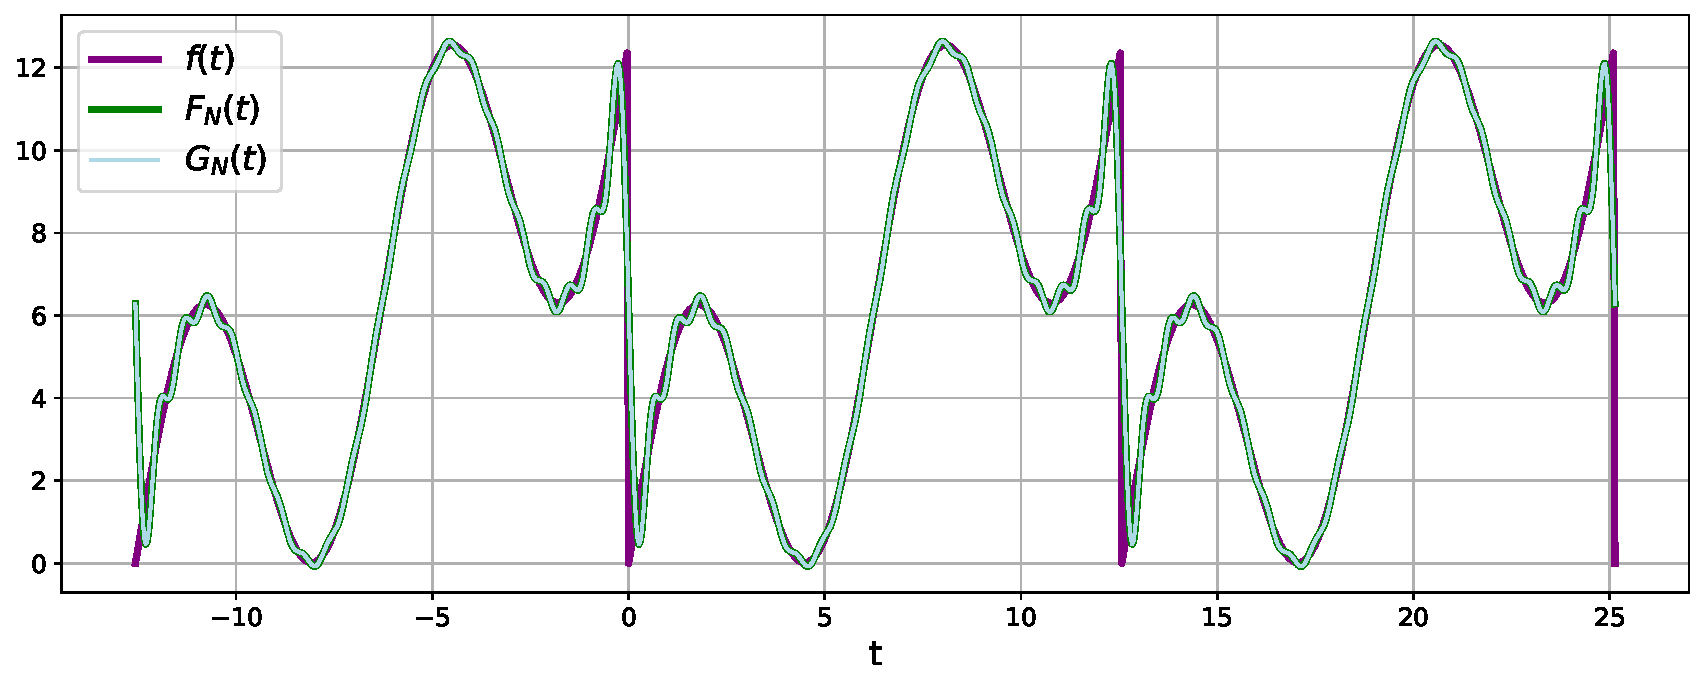
\includegraphics[width=1\textwidth]{images/graphs/figure_26.pdf}
    \caption{Графики $F_N(t)$ и $G_N(t)$ при N=20}
\end{figure}

\begin{figure}[H] 
    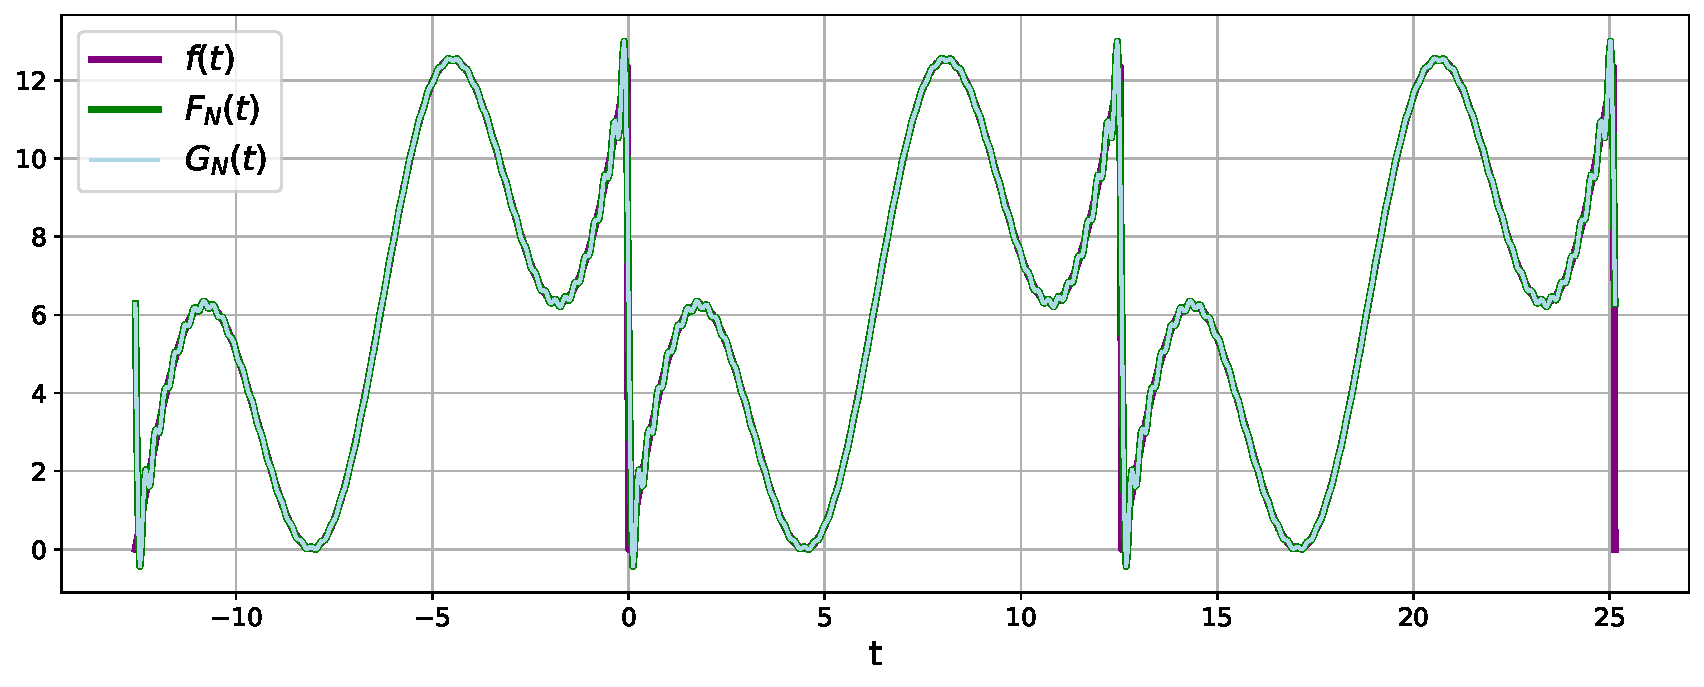
\includegraphics[width=1\textwidth]{images/graphs/figure_27.pdf}
    \caption{Графики $F_N(t)$ и $G_N(t)$ при N=50}
\end{figure}

\textbf{Проверка примерного равенства Парсеваля}

Для данной функции $f(t) = (1-\pi)^2 \sin(t) + t$ с периодом $T = 4\pi$ примерное равенство Парсеваля имеет вид:
\[
\frac{1}{4\pi}\int_{-4\pi}^{0} \left[(1-\pi)^2 \sin(t) + t\right]^2dt \approx \sum_{n=-N}^{N} |c_n|^2
\]

Проверим оценку для максимального рассмотренного $N = 50$:

\begin{table}[H]
\centering
\begin{tabular}{|l|c|}
\hline
\textbf{Величина} & \textbf{Значение} \\
\hline
Левая часть $\displaystyle\frac{1}{4\pi}\int_{-4\pi}^{0} \left[(1-\pi)^2 \sin(t) + t\right]^2dt$ & 53.982672 \\
Правая часть $\displaystyle\sum_{n=-50}^{50} |c_n|^2$ & 53.824261 \\
Абсолютная разница & $1.584 \times 10^{-1}$ \\
\hline
\end{tabular}
\caption{Проверка примерного равенства Парсеваля при $N = 50$}
\end{table}

\textbf{Анализ:} Для данной функции порядок ошибки на 1 меньше, чем значения левой и правой частей равенства.

\subsection{Выводы по заданию 1}
Команда отмечает медленную скорость выполнения расчётов при сравнительно небольших N, так как на каждом шаге программа должна считать два (в нашем случае) интеграла. Возможно этого можно было бы избежать, если самостоятельно реализовать численное интегрирование и лично контролировать частоту дискретизации при интегрировании.

Для оптимизации вычислений мы отказались от взятия экспоненциального интеграла и вместо этого выразили коэффициент комплексного разложения через вещественные коэффициенты. С одной стороны это бессмысленно из-за того, что мы не берём нужный интеграл, а как бы обходим его (спасибо математике), с другой стороны при проверке равенства Парсеваля гораздо удобнее считать сумму квадратов одного коэффициента, а не разных, чем мы и воспользовались.

При проверке примерного равенства Парсеваля мы столкнулись с тем, что получаются довольно разные ошибки. Они могут отличаться от значений левой и правой части равенства как на 1 порядок, так и на 5. Но сама величина ошибки может служить признаком контроля качества приближения функции частичными суммами. То есть в зависимости от целей, для которых испольуется приближение, могут быть допустимы разные ошибки: где-то важна точность до десятитысячных, а где-то достаточно десятых, но важна скорость.

% \subsection{Нечётная периодическая функция (Пилообразная волна)}
% В общем виде пилообразная волная задаётся следующим выражением:
% $$f(t) = \frac{2A}{T}\cdot t,\;\;\;t\in[-\frac{T}{2};\frac{T}{2}]$$

% Коэффициент А отвечает за амплитуду, T --- период. Тогда:
% $$f(t) = \frac{14t}{T}$$

% \begin{figure}[H]
%     \centering
%     
\includegraphics[width=0.5\linewidth]{images/figure_13.pdf}
%     % \caption{Caption}
%     \label{fig:placeholder}
% \end{figure}

\newpage
\section{Комплексная функция}

\subsection{Аналитическое выражение функции \( f(t) \)}

Согласно методичке, задана комплекснозначная периодическая функция с периодом \( T \) и параметром \( R > 0 \). Её действительная и мнимая части на одном периоде \( \left[-\frac{T}{8}, \frac{7T}{8}\right] \) определяются кусочно-линейными выражениями:

\[
\text{Re}(f(t)) =
\begin{cases}
R, & t \in \left[-\frac{T}{8}, \frac{T}{8}\right) \\
2R - \frac{8Rt}{T}, & t \in \left[\frac{T}{8}, \frac{3T}{8}\right) \\
-R, & t \in \left[\frac{3T}{8}, \frac{5T}{8}\right) \\
-6R + \frac{8Rt}{T}, & t \in \left[\frac{5T}{8}, \frac{7T}{8}\right)
\end{cases}
\]

\[
\text{Im}(f(t)) =
\begin{cases}
\frac{8Rt}{T}, & t \in \left[-\frac{T}{8}, \frac{T}{8}\right) \\
R, & t \in \left[\frac{T}{8}, \frac{3T}{8}\right) \\
4R - \frac{8Rt}{T}, & t \in \left[\frac{3T}{8}, \frac{5T}{8}\right) \\
-R, & t \in \left[\frac{5T}{8}, \frac{7T}{8}\right)
\end{cases}
\]

В работе приняты значения \( R = 4.0 \), \( T = 8.0 \). 




\begin{figure}[H]
    \centering
    
\includegraphics[width=0.7\linewidth]{images/sanini/figure_1.pdf}
    \caption{Параметрический график исходной функции f(t) на комплексной плоскости}
    \label{fig:placeholder}
\end{figure}



\newpage
\textbf{Ряд Фурье для комплексной функции}

Комплексный ряд Фурье имеет вид:
\[
G_N(t) = \sum_{n=-N}^N c_n e^{i\omega_n t}, \quad \omega_n = \frac{2\pi n}{T} 
\]

Коэффициенты \(c_n\) вычисляются по формуле:
\[
c_n = \frac{1}{T} \int_{-T/8}^{T/8} f(t)e^{-i\omega_n t}\, dt 
\]

\textbf{Численные значения коэффициентов при \(N = 2\)}

\[
\begin{aligned}
c_0 &= 0.0000 + 0.0000i \\
c_1 &= 4.5853 + 0.0000i \\
c_2 &= 0.0000 + 0.0000i 
\end{aligned}
\]


\subsection{Параметрические графики частичных сумм на комплексной плоскости}



\begin{table}[H]
    \centering
    \begin{tabular}{c c}
      
\includegraphics[width=0.9\textwidth]{images/sanini/figure_2.pdf}
    \end{tabular}
    % \caption{Caption}
    \label{tab:placeholder}
\end{table}

\begin{table}[H]
    \centering
    \begin{tabular}{c c}
\includegraphics[width=0.9\textwidth]{images/sanini/figure_3.pdf}  \\
    \end{tabular}
    % \caption{Caption}
    \label{tab:placeholder}
\end{table}

\begin{table}[H]
    \centering
    \begin{tabular}{c c}
      
\includegraphics[width=0.9\textwidth]{images/sanini/figure_4.pdf} 
    \end{tabular}
    % \caption{Caption}
    \label{tab:placeholder}
\end{table}

\begin{table}[H]
    \centering
    \begin{tabular}{c c}
\includegraphics[width=0.9\textwidth]{images/sanini/figure_5.pdf}  \\
    \end{tabular}
    % \caption{Caption}
    \label{tab:placeholder}
\end{table}


\newpage
\subsection{Графики вещественной и мнимой частей}

\begin{figure}[H]
    \centering
    
\includegraphics[width=1\linewidth]{images/sanini/figure_6.pdf}
    \caption{Вещественная и мнимая части комплексной функции \( f(t) \) и её приближения \( G_1(t) \) при \( N=1 \)}
    \label{fig:placeholder}
\end{figure}



\begin{figure}[H]
    \centering
    
\includegraphics[width=1\linewidth]{images/sanini/figure_7.pdf}
    \caption{Вещественная и мнимая части комплексной функции \( f(t) \) и её приближения \( G_2(t) \) при \( N=2 \)}
    \label{fig:placeholder}
\end{figure}



\begin{figure}[H]
    \centering
    
\includegraphics[width=0.9\linewidth]{images/sanini/figure_8.pdf}
    \caption{Вещественная и мнимая части комплексной функции \( f(t) \) и её приближения \( G_3(t) \) при \( N=3 \)}
    \label{fig:placeholder}
\end{figure}


\begin{figure}[H]
    \centering
    
\includegraphics[width=0.9\linewidth]{images/sanini/figure_9.pdf}
    \caption{Вещественная и мнимая части комплексной функции \( f(t) \) и её приближения \( G_4(t) \) при \( N=4 \)}
    \label{fig:placeholder}
\end{figure}



\subsection{Проверка примерного равенства Парсеваля}

Для комплексного ряда Фурье примерное равенство Парсеваля имеет вид:
\begin{equation}
\frac{1}{T} \int_{-T/8}^{T/8} |f(t)|^2 dt \approx \sum_{n=-N}^{N} |c_n|^2
\end{equation}

\begin{table}[H]
\centering
\begin{tabular}{|c|c|}
\hline
\textbf{Величина} & \textbf{Значение} \\
\hline
Левая часть $\displaystyle\int_{-T/8}^{T/8} |f(t)|^2 dt$ & 21.333344 \\
Правая часть $\displaystyle\sum_{n=-N}^{N} |c_n|^2$ & 21.329897 \\
Абсолютная разница & 3.45 $\times$ 10$^{-3}$ \\
\hline
\end{tabular}
\caption{Проверка примерного равенства Парсеваля при N = 10}
\end{table}

\textbf{Пояснение:} Для данной функции значение ошибки на 3 порядка меньше значений левой и правой частей



\subsection{Выводы по заданию 2}

\begin{itemize}
    \item Ряд Фурье эффективно аппроксимирует комплексную функцию. С увеличением числа членов ряда Фурье приближение становится более точным.
    \item Построены графики, на которых отображены исходная функция и её приближения, полученные с использованием ряда Фурье для различных значений \( N \).
    \item Параметрические графики на комплексной плоскости наглядно демонстрируют сходимость ряда по мере увеличения числа гармоник.
    \item Примерное равенство Парсеваля выполняется с ошибкой, на 3 порядка меньше, чем значения левой и правой частей.
\end{itemize}

\newpage
\section{Общий вывод}
Ряд Фурье аппроксимирует и вещественную, и комплексную функции с такой точностью, что при проверке примерного равенства Парсеваля при N = 10 ошибка всегда как минимум на 1 порядок меньше, чем значения левой и правой частей равенства. Делать какие-то выводы о размерности ошибки трудно, так как всё зависит в первую очердь от задач: где-то на первом месте будет стоять точность в конкретных величинах, например, на 5 порядков меньше самих значений, а где-то в приоритете будет производительность "лёгкой"\;аппроксимации.

С увеличением N увеличивается точность приближения частичных сумм Фурье к исходным функциям.


\newpage
\section{Приложение}
\subsection{Листинг к заданию 1}
\begin{minted}{python}
from scipy.integrate import quad
import numpy as np
import matplotlib.pyplot as plt

def save_separate_figures(extension="pdf", path=""):
    """ Saves each active matplotlib figure to a separate file. """
    # Получаем номера всех созданных фигур
    fig_nums = plt.get_fignums()

    for i in fig_nums:
        plt.figure(i)
        filename = f"figure_{i}.{extension}"
        plt.savefig(path+filename)
        print(f"Сохранен файл: {filename}")

def compute_fourier_coefficients(f, T, N, t0, out=True, disc_points=[]):
    """
    Считает коэффициенты для вещественного и комплексного рядов Фурье
    
    :param f: Функция вида f(t) = lambda t -> f(t, param1, param2 ...)
    :param T: Период функции
    :param N: Точность/количество членов ряда Фурье
    :param t0: Точка нижней границы периода функции (интегрируем от t0 до t0 + T)
    """
    a_arr = []
    b_arr = []
    c_arr_pos =[]
    c_arr_neg = []
    c_arr = []

    a0, _ = quad(f, t0, t0+T, points=disc_points)
    a0 *= 2/T
    c0 = a0/2
    # c_arr.append(c0)
    
    for n in range(1, N+1):
        omega_n = 2 * np.pi * n / T
        f_cos = lambda t: f(t) * np.cos(omega_n * t)
        f_sin = lambda t: f(t) * np.sin(omega_n * t)

        # Интегрируем
        temp_a_n, _ = quad(f_cos, t0, t0+T, points=disc_points, limit=100)
        temp_b_n, _ = quad(f_sin, t0, t0+T, points=disc_points, limit=100)

        c_n_pos = temp_a_n/T - temp_b_n*1j/T

        a_n = temp_a_n * 2/T
        b_n = temp_b_n * 2/T

        a_arr.append(a_n)
        b_arr.append(b_n)
        c_arr_pos.append(c_n_pos)
        c_arr_neg.append(np.conj(c_n_pos))
    c_arr_neg = c_arr_neg[::-1]
    c_arr = c_arr_neg + [c0] + c_arr_pos

    if out: 
        res = "[CFC] For real Fourier:\n"
        res += f"[CFC] a_0={a0:.2f}\n"
        for n in range(1, N+1):
            res += f"[CFC] a_{n}={a_arr[n-1]}; b_{n}={b_arr[n-1]}\n"
        res += "[CFC] For complex Fourier:\n"
        for n in range(-N, N+1):
            res += f"[CFC] c_{n}={c_arr[n+N]}\n"

        print(res)
    return (a0, a_arr, b_arr, c_arr)

def check_parseval(f, T, N, t0, out=True, disc_points=[]):
    """
    Проверяет равенство Парсеваля для функции f
    
    :param f: Функция вида f(t) = lambda t -> f(t, param1, param2 ...)
    :param T: Период функции
    :param N: Точность/количество членов ряда Фурье
    :param t0: Точка нижней границы периода функции
    """
    a0, a_arr, b_arr, c_arr = compute_fourier_coefficients(f, T, N, t0, out=False, disc_points=disc_points)
    
    f_squared = lambda t: f(t)**2
    left_part, _ = quad(f_squared, t0, t0+T, points=disc_points, limit=100)
    left_part /= T
    
    right_part_real = a0**2 / 4
    for n in range(len(a_arr)):
        right_part_real += (a_arr[n]**2 + b_arr[n]**2) / 2
    
    right_part_complex = 0
    for n in range(len(c_arr)):
        right_part_complex += np.abs(c_arr[n])**2
    
    if out:
        res = "\n[Parseval] Left part (integral): "
        res += f"{left_part:.6f}\n"
        res += f"[Parseval] Right part (real Fourier): {right_part_real:.6f}\n"
        res += f"[Parseval] Right part (complex Fourier): {right_part_complex:.6f}\n"
        res += f"[Parseval] Difference (real): {abs(left_part - right_part_real):.6e}\n"
        res += f"[Parseval] Difference (complex): {abs(left_part - right_part_complex):.6e}"
        print(res)
    
    return (left_part, right_part_real, right_part_complex)

def build_real_fourier(a0, a_n, b_n, T):
    """
    Функция для сборки вещественного ряда Фурье
    
    :param a0: коэффициент a_0
    :param a_n: массив коэффициентов a_n
    :param b_n: массив коэффициентов b_n
    :param T: период функции
    """
    if len(a_n) != len(b_n):
        raise Exception("a_n и b_n должны быть одной размерности")
    def F_N(t):
        result = a0/2
        for n in range(1, len(a_n) + 1):
            omega_n = 2 * np.pi * n / T
            result += a_n[n-1] * np.cos(omega_n * t) + b_n[n-1]*np.sin(omega_n*t)
        return result
    return F_N

def build_complex_fourier(c_n, T):
    N = (len(c_n)-1) // 2
    def G_N(t):
        result = 0
        for n in range(-N, N+1):
            omega_n = 2 * np.pi * n / T
            result += c_n[n + N] * np.exp(1j * omega_n * t)
        return np.real(result)
    return G_N

def draw_graphs(t, f, T, t0, N=[], disc_points=[], N2_title=""):
    """
    Рисует графики функций и их разложений Фурье (только если N != 2)
    
    :param t: Описание
    :param f: Описание
    :param T: Описание
    :param t0: Описание
    :param N: Описание
    """
    for n in N:
        out = n == 2 or n == max(N)
        if out: print(f"\n{N2_title}\nРазложение 2 порядка:")
        (a0, an, bn, cn) = compute_fourier_coefficients(f, T, n, t0, out=out, disc_points=disc_points)
        plt.figure()
        plt.grid()
        plt.plot(t, f(t), color="purple", label="Исходная функция", linewidth=3)
        if not out:
            plt.title(r"Графики $F_N(t)$ и $G_N(t)$" + f" при N={n}")
            F_N = build_real_fourier(a0,an,bn,T)
            G_N = build_complex_fourier(cn, T)
            plt.plot(t, F_N(t) , color="green", label=r"Вещественный ряд $F_N(t)$", linewidth=2,)
            plt.plot(t, G_N(t), color="lightblue", label=r"Комплексный ряд $G_N(t)$", linewidth=1)
            
        else:
            plt.title(N2_title)
            plt.xlabel("t", fontsize=15, labelpad=10)
            plt.grid(True)
            plt.axis('equal')

            plt.figure()
            plt.title(r"Графики $F_N(t)$ и $G_N(t)$" + f" при N={n}")
            plt.grid()
            plt.plot(t, f(t), color="purple", label="Исходная функция", linewidth=3)
            F_N = build_real_fourier(a0,an,bn,T)
            G_N = build_complex_fourier(cn, T)
            plt.plot(t, F_N(t) , color="green", label=r"Вещественный ряд $F_N(t)$", linewidth=2,)
            plt.plot(t, G_N(t), color="lightblue", label=r"Комплексный ряд $G_N(t)$", linewidth=1)
        

        
        plt.legend(loc="best")
        # plt.plot(t, t*[0])
        # plt.axvline(0)
        plt.xlabel("t", fontsize=15, labelpad=10)
        plt.grid(True)
        
        plt.axis('equal')



N_variations = [2, 3, 10, 20, 50]

def f1(t, t0, t1, t2, T, a, b):
    mod = (t - t0) % T + t0
    return np.where((mod >= t0) & (mod < t1), a, b)

a = 12
b = 6
t0 = 1
t1 = 2
t2 = 3
T1 = t2-t0

t_start = t0 - T1
t_end = t2 + T1

lambda_f1 = lambda t: f1(t, t0, t1, t2, T1, a, b)
t = np.linspace(t_start, t_end, 2000)

draw_graphs(t, lambda_f1, T1, t0, N=N_variations, disc_points=[t0, t1, t2], N2_title=f"Квадратная волна. T={T1:.2f}")


T2 = 6
t0 = -3
t1 = -2
t2 = -1
t3 = 1
t4 = 2
t5 = 3

def f2(tt, t0, t1, t2, t3, t4, t5, T):
    # Определяем, скаляр или массив
    is_scalar = np.isscalar(tt)
    
    # Приводим к массиву для единообразной обработки
    t_array = np.atleast_1d(tt)
    t_norm = ((t_array - t0) % T) + t0
    
    y = np.zeros_like(t_norm)
    
    # Применяем маски
    mask1 = (t_norm >= t0) & (t_norm < t1)
    y[mask1] = 4 * t_norm[mask1] + 12
    
    mask2 = (t_norm >= t1) & (t_norm < t2)
    y[mask2] = -2 * t_norm[mask2]
    
    mask3 = (t_norm >= t2) & (t_norm < t3)
    y[mask3] = 2
    
    mask4 = (t_norm >= t3) & (t_norm < t4)
    y[mask4] = 2 * t_norm[mask4]
    
    mask5 = (t_norm >= t4) & (t_norm < t5)
    y[mask5] = -4 * t_norm[mask5] + 12
    
    # Возвращаем скаляр, если на входе был скаляр
    return y.item() if is_scalar else y


t_start = t0 - T2
t_end = t5 + T2
t = np.linspace(t_start, t_end, 5000)

lambda_f2 = lambda t: f2(t, t0, t1, t2, t3, t4, t5, T2)
draw_graphs(t, lambda_f2, T2, t0, N=N_variations, disc_points=[t0, t1, t2, t3, t4, t5], N2_title=f"Котики T={T2:.2f}")



def f3(t, T, A):
  # + T/2 для того, чтобы остаток от деления был корректным
  # (с отрицательными работает по правилам кольца. здесь не подходит). потом возвращаем обратно
  t_norm = np.mod(t+T/2, T) - T/2
  return A*2/T * t_norm

T3 = 2*np.pi
t = np.linspace(-T3, T3*2, 1000)
a = 7

lambda_f3 = lambda t: f3(t, T3, a)

draw_graphs(t, lambda_f3, T3, t0=0, N=N_variations, N2_title=f"Пилообразная волна T={T3:.2f}")
check_parseval(lambda_f3, T3, N=max(N_variations), t0=0, out=True)
def f4(t, T, a):
  t = np.mod(t, T)
  return (1-np.pi)**2*np.sin(a*t) + t
T4=4*np.pi
a = 1

lambda_f4 = lambda t: f4(t, T4, a)

t = np.linspace(-T4, T4*2, 1000)
draw_graphs(t, lambda_f4, T4, t[0], N_variations, N2_title=f"Биение T={T4:.2f}")
check_parseval(lambda_f4, T4, N=max(N_variations), t0=t[0], out=True)

# save_separate_figures(path="/Users/itskifpetya/dev/freq_methods/lab1/graphs/")
plt.show()





\end{minted}
\label{app:task1}

\subsection{Листинг к заданию 2}
\begin{minted}{python}
import numpy as np
import matplotlib.pyplot as plt
import warnings
import os

warnings.filterwarnings('ignore')

def save_separate_figures(extension="pdf", path=""):
    """ Saves each active matplotlib figure to a separate file. """
    os.makedirs(path, exist_ok=True)
    fig_nums = plt.get_fignums()

    for i in fig_nums:
        plt.figure(i)
        filename = f"figure_{i}.{extension}"
        plt.savefig(os.path.join(path, filename))
        print(f"Сохранен файл: {filename}")


R = 4.0
T = 8.0
omega0 = 2 * np.pi / T

N_values = [1, 2, 3, 10]
N_max = max(N_values)

plt.rcParams.update({'font.size': 14})


def complex_function(t):
    t_shifted = (t + T/8) % T - T/8
    re = np.zeros_like(t_shifted)
    im = np.zeros_like(t_shifted)

    mask1 = (-T/8 <= t_shifted) & (t_shifted < T/8)
    mask2 = (T/8 <= t_shifted) & (t_shifted < 3*T/8)
    mask3 = (3*T/8 <= t_shifted) & (t_shifted < 5*T/8)
    mask4 = (5*T/8 <= t_shifted) & (t_shifted < 7*T/8)

    re[mask1] = R
    im[mask1] = 8 * R * t_shifted[mask1] / T
    re[mask2] = 2*R - 8 * R * t_shifted[mask2] / T
    im[mask2] = R
    re[mask3] = -R
    im[mask3] = 4*R - 8 * R * t_shifted[mask3] / T
    re[mask4] = -6*R + 8 * R * t_shifted[mask4] / T
    im[mask4] = -R

    return re + 1j * im


def compute_coeffs(func, N_max):
    M = 10000
    t_points = np.linspace(0, T, M, endpoint=False)
    dt = t_points[1] - t_points[0]
    f_values = func(t_points)
    coeffs = np.zeros(2* N_max + 1, dtype=complex)
    for n in range(-N_max, N_max + 1):
        idx = N_max + n
        exp_values = np.exp(-1j * n * omega0 * t_points)
        coeffs[idx] = np.sum(f_values * exp_values) * dt / T
    return coeffs


coeffs = compute_coeffs(complex_function, N_max)


t_plot = np.linspace(0, 2*T, 2000)
f_plot = complex_function(t_plot)

def partial_sum(t, coeffs, N):
    G_N = np.zeros_like(t, dtype=complex)
    N_total = (len(coeffs) - 1) // 2
    for n in range(-min(N, N_total), min(N, N_total) + 1):
        idx = N_total + n
        G_N += coeffs[idx] * np.exp(1j * n * omega0 * t)
    return G_N

# Построение графика исходной функции
plt.figure(figsize=(10, 8))
plt.plot(f_plot.real, f_plot.imag, 'b-', linewidth=2, label='$f(t)$', alpha=0.8)
plt.title(f'Параметрический график исходной функции f(t)', fontsize=18)
plt.grid(True, alpha=0.3)
plt.legend(fontsize=14, loc='upper right')
plt.axis('equal')
plt.xlim([-R*1.2, R*1.2])
plt.ylim([-R*1.2, R*1.2])
plt.tight_layout()


# Построение параметрических графиков на комплексной плоскости
for N in N_values:
    G_N = partial_sum(t_plot, coeffs, N)

    plt.figure(figsize=(10, 8))
    plt.plot(f_plot.real, f_plot.imag, 'b-', linewidth=2, label='$f(t)$', alpha=0.8)
    plt.plot(G_N.real, G_N.imag, 'r--', linewidth=2, label=f'$G_{N}(t)$')
    plt.xlabel('Re', fontsize=16)
    plt.ylabel('Im', fontsize=16)
    plt.title(f'Параметрический график, $N={N}$', fontsize=18)
    plt.grid(True, alpha=0.3)
    plt.legend(fontsize=14, loc='upper right')
    plt.axis('equal')
    plt.xlim([-R*1.2, R*1.2])
    plt.ylim([-R*1.2, R*1.2])
    plt.tight_layout()


# Построение вещественной и мнимой частей отдельно для каждого N
for N in N_values:
    G_N = partial_sum(t_plot, coeffs, N)
    fig, (ax1, ax2) = plt.subplots(2, 1, figsize=(12, 8))
    # График вещественной части
    ax1.plot(t_plot, f_plot.real, 'b-', linewidth=2, label='Re($f(t)$)', alpha=0.8)
    ax1.plot(t_plot, G_N.real, 'r--', linewidth=2, label=f'Re($G_{N}(t)$)')
    ax1.set_xlabel('$t$', fontsize=16)
    ax1.set_ylabel('Re', fontsize=16)
    ax1.set_title(f'Вещественная часть, $N={N}$', fontsize=18)
    ax1.grid(True, alpha=0.3)
    ax1.legend(fontsize=14)
    ax1.set_xlim([0, 2*T])
    # График мнимой части
    ax2.plot(t_plot, f_plot.imag, 'g-', linewidth=2, label='Im($f(t)$)', alpha=0.8)
    ax2.plot(t_plot, G_N.imag, 'm--', linewidth=2, label=f'Im($G_{N}(t)$)')
    ax2.set_xlabel('$t$', fontsize=16)
    ax2.set_ylabel('Im', fontsize=16)
    ax2.set_title(f'Мнимая часть, $N={N}$', fontsize=18)
    ax2.grid(True, alpha=0.3)
    ax2.legend(fontsize=14)
    ax2.set_xlim([0, 2*T])

    plt.suptitle(f'Вещественная и мнимая части $N={N}$: ', fontsize=20)
    plt.tight_layout()
    #plt.show()

# Вычисление левой части равенства Парсеваля
t_parseval = np.linspace(0, T, 10000, endpoint=False)
dt_parseval = t_parseval[1] - t_parseval[0]
f_parseval = complex_function(t_parseval)
left_parseval = np.sum(np.abs(f_parseval)**2) * dt_parseval / T

# Вычисление правой части равенства Парсеваля
N_parseval = N_max
c_parseval = coeffs[N_max - N_parseval : N_max + N_parseval + 1]
right_parseval = np.sum(np.abs(c_parseval)**2)

print(left_parseval)
print(right_parseval)

plt.show()
#save_separate_figures("pdf", r"C:\Users\alexb\OneDrive\Рабочий стол\итмо\ЧМ\lab1\картинки")
\end{minted}
\label{app:task2}

\end{document}
